\chapter{Evaluation}
This chapter evaluates the research performed during the PhD.

The case studies both led to significant improvements to the measured reliability of the treatment app. 

For the Kiwix project this reduction was one of the main reasons why they then chose to update the codebase for the majority of their custom apps~\footnote{The Kiwix project team decided some seldom used apps were not worth updating.}. They achieved similar improvements in the measured reliability despite only using the default analytics provided by Google Play Console. 

For the Catrobat project the development teams chose to add crash and mobile analytics to their iOS app which had neither previously and mobile analytics to their Android app, as it already incorporated crash analytics.

\section{Evaluation of the Kiwix case study}
%%%% Table generated originally by Spread-LaTeX
%\begin{adjustwidth}{-1 cm}{-1 cm}
\begin{threeparttable}[!htp]\centering
\caption{Reductions in Crash Rates}\label{tab:evaluation-reductions-in-crash-rates}
\scriptsize
\begin{tabularx}\textwidth{lrrr} % SHOULD-DO I'd like to reduce the width slightly.
\toprule
%& & & & \\
&\multicolumn{3}{c}{30-day crash rates reported in Android Vitals~\tnote{0}} \\
\midrule
\multirow{2}{*}{.} &\multicolumn{2}{c}{Kiwix Apps} \\
Stage &Release&\cellcolor[HTML]{efefef}Experiment &Control  \\

&\cellcolor[HTML]{efefef}&\cellcolor[HTML]{efefef}Kiwix & WikiMed English \\

1 &0 
  &\cellcolor[HTML]{efefef}5.07\% &1.13\% \\
2 &1 &\cellcolor[HTML]{efefef}3.12\%~\tnote{1} &\multirow{2}{*}{\cellcolor[HTML]{A8A8A8}}... \\
3 &2~\tnote{2} &\cellcolor[HTML]{efefef}1.59\%~\tnote{3} & \cellcolor[HTML]{A8A8A8}... \\
  &3 &\cellcolor[HTML]{efefef}0.53\%~\tnote{4} &1.09\%~\tnote{5} \\
4 &4 &\cellcolor[HTML]{efefef}0.72\%~\tnote{6} &0.60\%~\tnote{7} \\
  &4~\tnote{8} 
&\cellcolor[HTML]{efefef}0.55\% &0.41\% \\
  &5 &\cellcolor[HTML]{efefef}0.40\%~\tnote{9} &0.26\%~\tnote{10} \\
\bottomrule
\end{tabularx}
\begin{tablenotes}
  \item[0] Except when otherwise noted.
  \item[1] Kiwix Release 2.5 with the previous custom download facility replaced by a Google Android downloader.
  \item[2] The code is under 25 lines including 10 lines of comments~\url{https://github.com/kiwix/kiwix-android/pull/1388}.
  \item[3] Aggregate crash rate over 7 days for versions 2.4, 2.5.1, 2.5.2, 2.5.3 (to Aug \nth{26} 2019).
  \item[4] Previous 30 days crash rate, before release 3.1.2 pushed the crash rate up (same graph as TODO).
  \item[5] \emph{Unchanged release from the first control.}
  \item[6] Includes 3.1.2 which had an average (mean) crash rate of roughly 1.7\% (roughly \nth{31} Dec 2019).
  \item[7] A mixed set of crash rates, averaged by Android Vitals. For the first updated release of Wikimed (the 2019-12 release).
  \item[8] As usage increased of the more reliable releases the averages declined.
  \item[9] The crash rates for releases 3.2.1 are 0.23\% and 3.3.1 are 0.31\%
  \item[10] Release 2020-03 actually has a crash rate of around 0.05\% the numbers are higher as there are still significant volumes of usage on the previous 2 releases.

\end{tablenotes}
\end{threeparttable}
%\end{adjustwidth}
\vspace{5mm}
%%%% Isabel recommends creating a timeline instead - sounds good SHOULD-DO

Table~\ref{tab:evaluation-reductions-in-crash-rates} provides a numerical summary of five releases of two of the Kiwix Android apps. There are four stages in this case study:

\begin{enumerate}
    \itemsep0em
    \item The baseline
    \item Simplifying the most buggy code
    \item Applying the concepts in the research to the experiment
    \item The new normal: %ongoing improvements to the experiment app \emph{and} applying these improvements to the custom apps (including the previous control app).
\end{enumerate}
% Great ideas to reduce space in list items in https://tex.stackexchange.com/questions/6081/reduce-space-between-enumerated-items
% COULD-DO I've only applied the basic suggestion for this single list so far, might be worth thesis wide changes as the thesis matures.

The active part of the experiment started in stage 3 of this case study, although the initial research into the feasibility started several months earlier during the baseline stage.

\subsection{Stage 1: the baseline}
Before the experiment started there was little focus on finding and fixing causes of crashes. The development team did fix some sporadically, however they seldom used the reports from Android Vitals to identify crashes or address them.

The core app included an integrated download facility to download content to a user's local device. Files sizes ranged from a few MB to over 60GB and could take several days to download, especially in areas where connectivity wasn't ideal.  This integrated download facility provided users with several useful features, for example, they could pause and restart downloads. It also had an integrated recovery mechanism to restart and continue partial downloads after a failure, and it provided users with a progress indicator. However, this custom download facility had numerous bugs and was the largest source of crashes in real world use.

The custom apps were pre-packaged with content (which Google Play Services downloaded at the same time as downloading the app's binary). They did not need, and did not include the custom downloader. This meant their crash rates were significantly better (lower) than the core app managed.

\subsection{Stage 2: simplifying the most buggy code}
The first release, release 1 in the table, predated the hackathon (which was the start of the experiment). In this release the lead developer decided to replace a large body of custom code with generic downloader code rather than focus on fixing individual sections of code. The custom code was considered too problematic to fix. However, there was a trade-off by increasing the reliability there was a reduction in usability and also an impact on what happened when downloads stopped or otherwise failed before completion.

\subsection{Stage 3: applying the research concepts of the experiment app}
I convinced the the leaders of the Kiwix project that we might be able to reduce the crash rate significantly by applying the concepts described in chapter 5. They had slowly become increasingly aware of the excessively high crash rate and the potential impact on both users and the app store's ranking of the apps based on the high crash rates. 

We agreed we would start by focusing on several of the most frequently occurring crashes as reported in Android Vitals. The opportunity to do so was at a week-long hackathon in Stockholm in August 2019. I led the discussions and analysis with several of the volunteer developers at the hackathon. 

Following this discussion and analysis about the crashes being reported in Android Vitals for version \texttt{2.5.0} of the core application, the developers fixed several of the causes of the most frequent crashes with a surprisingly small amount of code of under 25 lines (including 10 lines of text added to the release log)\footnote{\url{https://github.com/kiwix/kiwix-android/pull/1388}}.

Various developers continued to make corrective changes to the codebase which made ongoing incremental improvements to the app released to the \texttt{2.5.x} releases. 

\subsection{Stage 4: the new normal}
The improvements in the reliability of the core app were sufficiently compelling \emph{and} the reliability of the custom apps sufficiently poor that the development team chose to refresh the majority of the custom apps, including the one used as the control (WikiMed English). Note: Various details of the crash rate at the time and the plan to migrate the custom apps are included in~\url{https://github.com/kiwix/kiwix-android/issues/1426}. 

All the apps share a common codebase, they are created using a common set of build scripts, they differ in their data contents, various `resources'~\footnote{\emph{``Resources are the additional files and static content that your code uses, such as bitmaps, layout definitions, user interface strings, animation instructions, and more."}~\url{https://developer.android.com/guide/topics/resources/providing-resources}}, and the custom apps exclude file management and download features as the contents are pre-packaged as part of the build process instead.

Several releases later, each with various changes and improvements aimed at fixing causes of crashes the crash rate was materially lower than when we started, at the time of writing the overall crash rate for the last 7 days is 0.54\% which is inflated because the rash rate for the previous release (\texttt{3.1.2}) spiked at 1.38\%, compared to 0.18\% for release (\texttt{3.0.5} -  the last production release) and 0.25\% for the recently released fix (\texttt{3.1.3}).

\subsection{Overall evaluation of the Kiwix case study}
Within five months the project was able to reduce the crash rate of the core application from over 3\% to around a tenth of that figure. One of the main causes was the focus on addressing the most prevalently reported crash clusters in Android Vitals. This was not the only cause, the software was also being revised and updated, this included replacing some of the existing Java code with Kotlin equivalents. 

Empirical research in Android apps that migrate from Java to Kotlin indicate the code quality often improves in tandem according to static analysis of the binary files of various releases of the studied opensource apps~\cite{GoisMateus2019_an_empirical_study_on_the_quality_of_android_apps_in_kotlin}. That work does not investigate exceptions or crashes, it does include the Kiwix Android project~\footnote{Kiwix is listed as one of the projects their research investigated:~\url{https://github.com/UPHF/kotlinandroid/blob/master/docs/fdroid_all.md}.}. However, their research predates both my case study and when the Kiwix codebase transitioned to Kotlin.

The Kiwix Android project team continue to file bug reports and address them, for instance {\small~\href{https://github.com/kiwix/kiwix-android/issues/2104}{\texttt{github.com/kiwix/kiwix-android/issues/2104}}} 
provides an example of the lead developer raising a bug report for a crash reported by Android Vitals; and \\{\small ~\href{https://github.com/kiwix/kiwix-android/issues?q=is\%3Aissue+\%22crash+report\%22+}{\texttt{github.com/kiwix/kiwix-android/issues?q=is\%3Aissue+\%22crash+report\%22+}}} provides an up-to-date view of issues labeled with ``crash report". 

In conclusion, addressing crash reports is now performed actively by the developers and the crash rate of all the Android apps updated since the start of the case study have improved.

\section{Evaluation of the Catrobat case study}
The developers were able to significantly improve the reliability of their major Android app: Pocket Code, through applying a variation of the process identified in my research. The minor app, called Pocket Paint, is a separately packaged version of the drawing (paint) functionality in Pocket Code.

The project team were able to use two sources of analytics on crashes: Google Play Console incorporating Android Vitals, and Fabric Crashlytics. There were differences in the outputs and results of these tools, these are discussed later in this chapter, nonetheless they contained a common set of crashes and fixing the crash was reflected in both tools.

The project has a particularly and unusually mature process and focus on software quality as part of being an essential year-long module for various undergraduate courses and also used for post graduate research at Masters and PhD level. Nonetheless the crash rate was stubbornly high and exceeded Google's limit before we started the case study.

TBC

Still to do:
\begin{itemize}
    \item Intermittent focus on addressing crashes
    \item Loss of Crashlytics data for a period through a mistake configuring a release.
    \item The inclusion of Firebase Analytics in the Android app.
    \item The inclusion of Crash and Firebase Analytics in the iOS app, including ongoing work: See Firebase in iOS app https://jira.catrob.at/browse/CATTY-371?jql=text%20~%20%22firebase%22%20ORDER%20BY%20created%20DESC 
    \item Proposal to move to privacy-friendly analytics tools. 
\end{itemize}



\section{Evaluation of the Analytics Tools}

\textbf{TODO} \textit{Rewrite this section using the evaluation criteria in Chapter 5.}

The research primarily used and compared two analytics tools: Google Play Console incorporating Android Vitals, and Fabric Crashlytics, developed and maintained by Google. The research identified a wide range of flaws, summarised here.

\begin{enumerate}
    \item Testing discouraged: being encouraged and able to test the workings of the algorithm can increase the confidence in the analytics being generated. Flaws can be identified, discussed and either addressed or workarounds found.
    \item Negative user populations: Google Play Console provides two complementary graphs in addition to a third value useful for triangulation and for understanding the user-base for an app. For some apps the combination of the data in the first two graphs adds up to a negative volume of users.
    \item Gaps in the data: On numerous occasions Android Vitals graphs had gaps in the charts.
    \item No updates for 10+ days: in Autumn 2019. No explanation or information was provided to developers about the problem or the causes. %pigeon food experiment psychological effects.
    \item No service dashboard: Google Play Console does not provide anywhere to check the current status or previous outages (unlike many other similar tools and other Google services).
    \item Repeated graphs in dashboard report.
    \item Inconsistent data ranges for some of the graphs in the dashboard report.
    \item Incorrect data ranges for Crash and ANR statistics reports.
    \item Unexplained and unfounded headline warning alerts.
    \item Missing URL parameters for links to drill-down reports in Android Vitals for some Android Releases.
    \item Second most popular country's details conflated with the the most popular and used for the title of one of the acquisition reports.
    \item Poor grouping of crash clusters.
    \item Lack of reports for low to medium volume user-bases.
    \item 10x difference in calculated crash rate between the two analytics tools.
\end{enumerate}

% Group into types of problem. 

\iffalse 
\begin{table}[!htbp]
    \begin{threeparttable}[t]
    \footnotesize
    \centering

    \begin{tabular}{p{0.15\textwidth}p{0.3\textwidth}p{0.4\textwidth}}
    Flaw &Example &Impact \\
    \hline

    Negative populations &
    Pocket Code (see lifetime report L) &
    Lack of trust in Google’s analytics.\\
    
    Gaps in the data &
    Data missing for 1+ days (see below for examples) &
    Calculations affected, reduction in value of the reports, incomplete information. \\
    
    Missing URL parameters &
    Links to drill down on crash clusters for particular Android versions\tnote{1} &
    Confusion, risk of misattributing the reported crashes to a particular Android version when they are actually for the overall, current range of Android releases an app is running on. \\
    
    Incorrect ranges (a possible off-by-one calculation?) &
    Mismatch between overview and timeseries reports for Crashes and ANRs (see figures W,X,Y,Z). \\
    
    Poor groups of crash clusters &
    Kiwix examples dated \nth{4} July 2020\tnote{2} &
    Flaws in bug identification (mistakenly believing the scope of a crash cluster), potential suboptimal prioritisation of bugs to address. \\
    
    Lack of reports for low-volumes of usage &
    e.g. for WikiMed in Japanese with 1842 active users &
    Some key reports not available during early growth stages of an app, those apps may fail to thrive if they’re failing and developers don’t know the causes are poor reliability. \\
    
    \nth{2} country’s data conflated with \nth{1} &
    Acquisition Reports in app dashboard (see screenshot C)\tnote{3} &
    Confusion and lack of confidence in the reports. \\
    
    No facility for testing and testing discouraged &
    Implicit from the Terms of Service, section\tnote{4}. Other analytics tools, including those provided by Google, do encourage testing. &
    Developers dissuaded from testing the functionality or reporting. They have to [decide whether to] take on trust what Google chooses to tell them. \\


    \end{tabular}
    \begin{tablenotes}
    \item[1]e.g. the URL includes the relevant numeric value for most but not all the Android Versions \texttt{androidVersion=28} is correct and present for Android 8.1
    
    \item[2] a) \texttt{java.lang.IllegalStateException org.kiwix.kiwixmobile.core.base.BaseActivity.onCreate} \\
    b) \texttt{tgkill}
    
    \item[3] Note: partly addressed in the June 2020 revamp of Google Play Console.
    
    \item[4] \emph{``Broken Functionality We don’t allow apps that crash, force close, freeze, or otherwise function abnormally.”}~\cite{google_play_developer_policy_center}
    \end{tablenotes}
    
    \caption{Issues in Google Play Console Reports}
    \label{tab:issues-in-google-play-console-reports}
    \end{threeparttable}
\end{table}
\fi

% Please add the following required packages to your document preamble:
% \usepackage{booktabs}
% \usepackage[normalem]{ulem}
% \useunder{\uline}{\ul}{}
\begin{table}[!htbp]
\scriptsize
\renewcommand\TPTminimum{\textwidth}
%% Arrange for "longtable" to take up full width of text block
\setlength\LTleft{0pt}
\setlength\LTright{0pt}
\setlength\tabcolsep{6pt}
\begin{tabular}{p{0.18\textwidth}p{0.38\textwidth}p{0.4\textwidth}} %{@{}lll@{}}

\toprule
Flaw &
  Example &
  Impact \\ \midrule
Negative populations &
  Pocket Code (see lifetime report below) &
  Lack of trust in Google’s analytics \\
Gaps in the data &
  Data missing for 1+ days (see below for examples) &
  Calculations affected, reduction in value of the reports, incomplete information \\
Missing URL parameters &
  Links to drill down on crash clusters for particular Android versions e.g. Android 8.0 vs. Android 8.1 &
  Confusion, risk of misattributing the reported crashes to a particular Android version when they are actually for the overall, current range of Android releases an app is running on. \\
Incorrect ranges (a possible off-by-one calculation) &
  Mismatch between overview and timeseries reports for Crashs and ANRs (see below for examples - 4 figures) &
  One day’s data ‘missing’ from the timeseries reports. Confusion, lack of trust in the reports. \\
Poor groups of crash clusters &
  Kiwix example 04 Jul 2020\\ java.lang.IllegalStateException &
  Flaws in bug identification (mistakenly believing the scope of a crash cluster), potential suboptimal prioritisation of bugs to address. \\
Lack of reports for low-volumes of usage &
  E.g. for WikiMed in Japanese with 1842 active users. &
  Some key reports not available during early growth stages of an app, those apps may fail to thrive if they’re failing and developers don’t know the causes are poor reliability \\
2nd country’s data conflated with 1st. &
  Acquisition Reports in app dashboard (see below for screenshots). Note partly addressed in the June 2020 revamp of Google Play Console. &
  Confusion and lack of confidence in the reports \\
No facility for testing and testing discouraged &
  Implicit from the Terms of Service, section “Broken Functionality We don’t allow apps that crash, force close, freeze, or otherwise function abnormally.” Other analytics tools, including those provided by Google, do encourage testing. &
  Developers dissuaded from testing the functionality or reporting. They have to {[}decide whether to{]} take on trust what Google chooses to tell them. \\
Repeated graphs &
  In dashboard report for apps 2 graphs are repeated: New users acquired, and Users lost. &
  Breaks ‘don’t repeat yourself’ (DRY). Waste of attention. \\
Inconsistent date ranges for some dashboard reports &
  The audience growth reports: new users acquired by country, and top countries graphs are for fixed periods - the period is not explained or visible on the report. In contrast the Android Vitals graphs are explicitly for the last 30 days, not necessarily ideal but at least documented that the period is fixed. &
  Confusion, inconsistent behaviour of the reports, potential for misinterpretation. \\
No updates for several days &
  In September 2019 the Android Vitals graphs and data were not updated for around 10 days &
  Inability to see or respond to stability issues, loss of confidence in the service. \\
Unexplained negative headline rate &
  Crash rate of 1.66\% - urgent warning, yet drilling down into the report none of the details reach 1.66\%, they are all significantly lower values. &
  Reduction in confidence in their alerts, and similarly a lack of trust in their calculations \\
No Service Problem Reporting &
  Google, and many others, provide a service status page, and many also include a history. For instance Salesforce provides https://trust.salesforce.com/en/ and status pages e.g. https://status.salesforce.com/incidents/5800 &
  A lack of transparency which leads to a lack of trust. \\ \bottomrule
\end{tabular}
    \caption{Issues in Google Play Console Reports}
    \label{tab:issues-in-google-play-console-reports}
\end{table}


\section{Evaluation of the software created for the research}

Placeholders for this section:
\begin{itemize}
    \item Testing logging:
    \item Zipternet app: Microsoft AppCenter, zero-to-ten, Kotlin.
    \item Vital Scraper and related projects: NPM package release process.
    \item ...
\end{itemize}



\section{Validity considerations}
In absolute terms, my research covers a minuscule percentage of all the apps available in Google Play, roughly 1 in 100,000. So these results may not apply to all the apps, or potentially even a majority of them. And yet, the results have consistently indicated that when development teams pay attention to stability metrics they are able to materially improve the reliability of their mobile apps even though their apps range across several app store categories and range in userbase from under 1,000 active users to over 160,000. These apps are spread across 6 of the 7 groups of downloads identified in AppBrain's `Download distribution of Android apps'~\cite{appbrain_download_statistics_june_2019} and similarly 5 of the 7 groupings representing over 94\% of the distribution of downloads in Google Play according to Wang ~\emph{et al} (2018)~\cite{wang2018beyond}.

\textbf{MUST-DO} answer the following question: What exists in the literature, common practices, vs what I was able to achieve. \emph{From a question raised by Alistair Willis, OU, 30 April 2020.}

\subsection{How many developers are enough to ask?}
On of the key considerations for research is adequacy in terms of coverage. For my research there are several types of coverage, including: development teams, user-bases for the various apps, software tech stacks used (in terms of programming languages, analytics libraries, etc.), application domains, and so on. 

c.f. Krug is a well respected Usability guru whose work is inherently practical in nature. In the first edition of his~\emph{``Don't make me Think"} book he discusses ways to obtain practical results even with short timescales and few resources. In terms of obtaining value the author indicated that 3 to 4 people were capable of delivering more relevant feedback by involving them over time, (Chapter 9 in ~\cite{krug2000dont_make_me_think}). In terms of selecting the candidates his recommendation was to worry less about selecting 'representative users', instead\emph{``Recruit loosely, and grade on a curve."} (Chapter 9 in ~\cite{krug2000dont_make_me_think})~\footnote{Note: Krug made several chapters, including this one available online when the second edition of the book was published. I have copies of all three versions of the book and of these chapters as PDF files.}.

% exploratory personas.
% GTAC conference talk about developers not having engineering degrees (The one Isabel went to Mr Tupule, Googler.)

My research included working with two mature project teams and developers of three commercial apps. It is also based on work I did in industry that predates the PhD research, unfortunately I am not able to provide details of those projects in my thesis. 

\section{Summary of evaluation of case studies}


Much remains to do in the area of applying mobile analytics to the development practices. Real-world bugs, including several I experienced recently and described next are not likely to be detected by the developers without a combination of some of all of: improved testing practices, rich in-app feedback, and using and applying in-app mobile analytics.

A couple of examples of poor user experiences that don't involve crashes or freezes (so would not be detected using the platform-level analytics) are, the Financial Times Android app: Figure~\ref{fig:ft_android_app_bsod}, and The Times newspaper iOS app: ``Cannot find article: Apologies, this article no longer exists." Figure~\ref{fig:thetimes-ios-this-article-no-longer-exists}. Of these, the missing article could be recorded easily using in-app error reporting (it might be detected by a non-fatal exception using a crash-reporting library or mobile analytics). The black screen is likely to be harder to report on (as if the developers were aware of the potential for the problem they could add error-handling and error-recovery logic).

\begin{figure}[!tbp]
    \centering
    \subfloat[What the user sees] {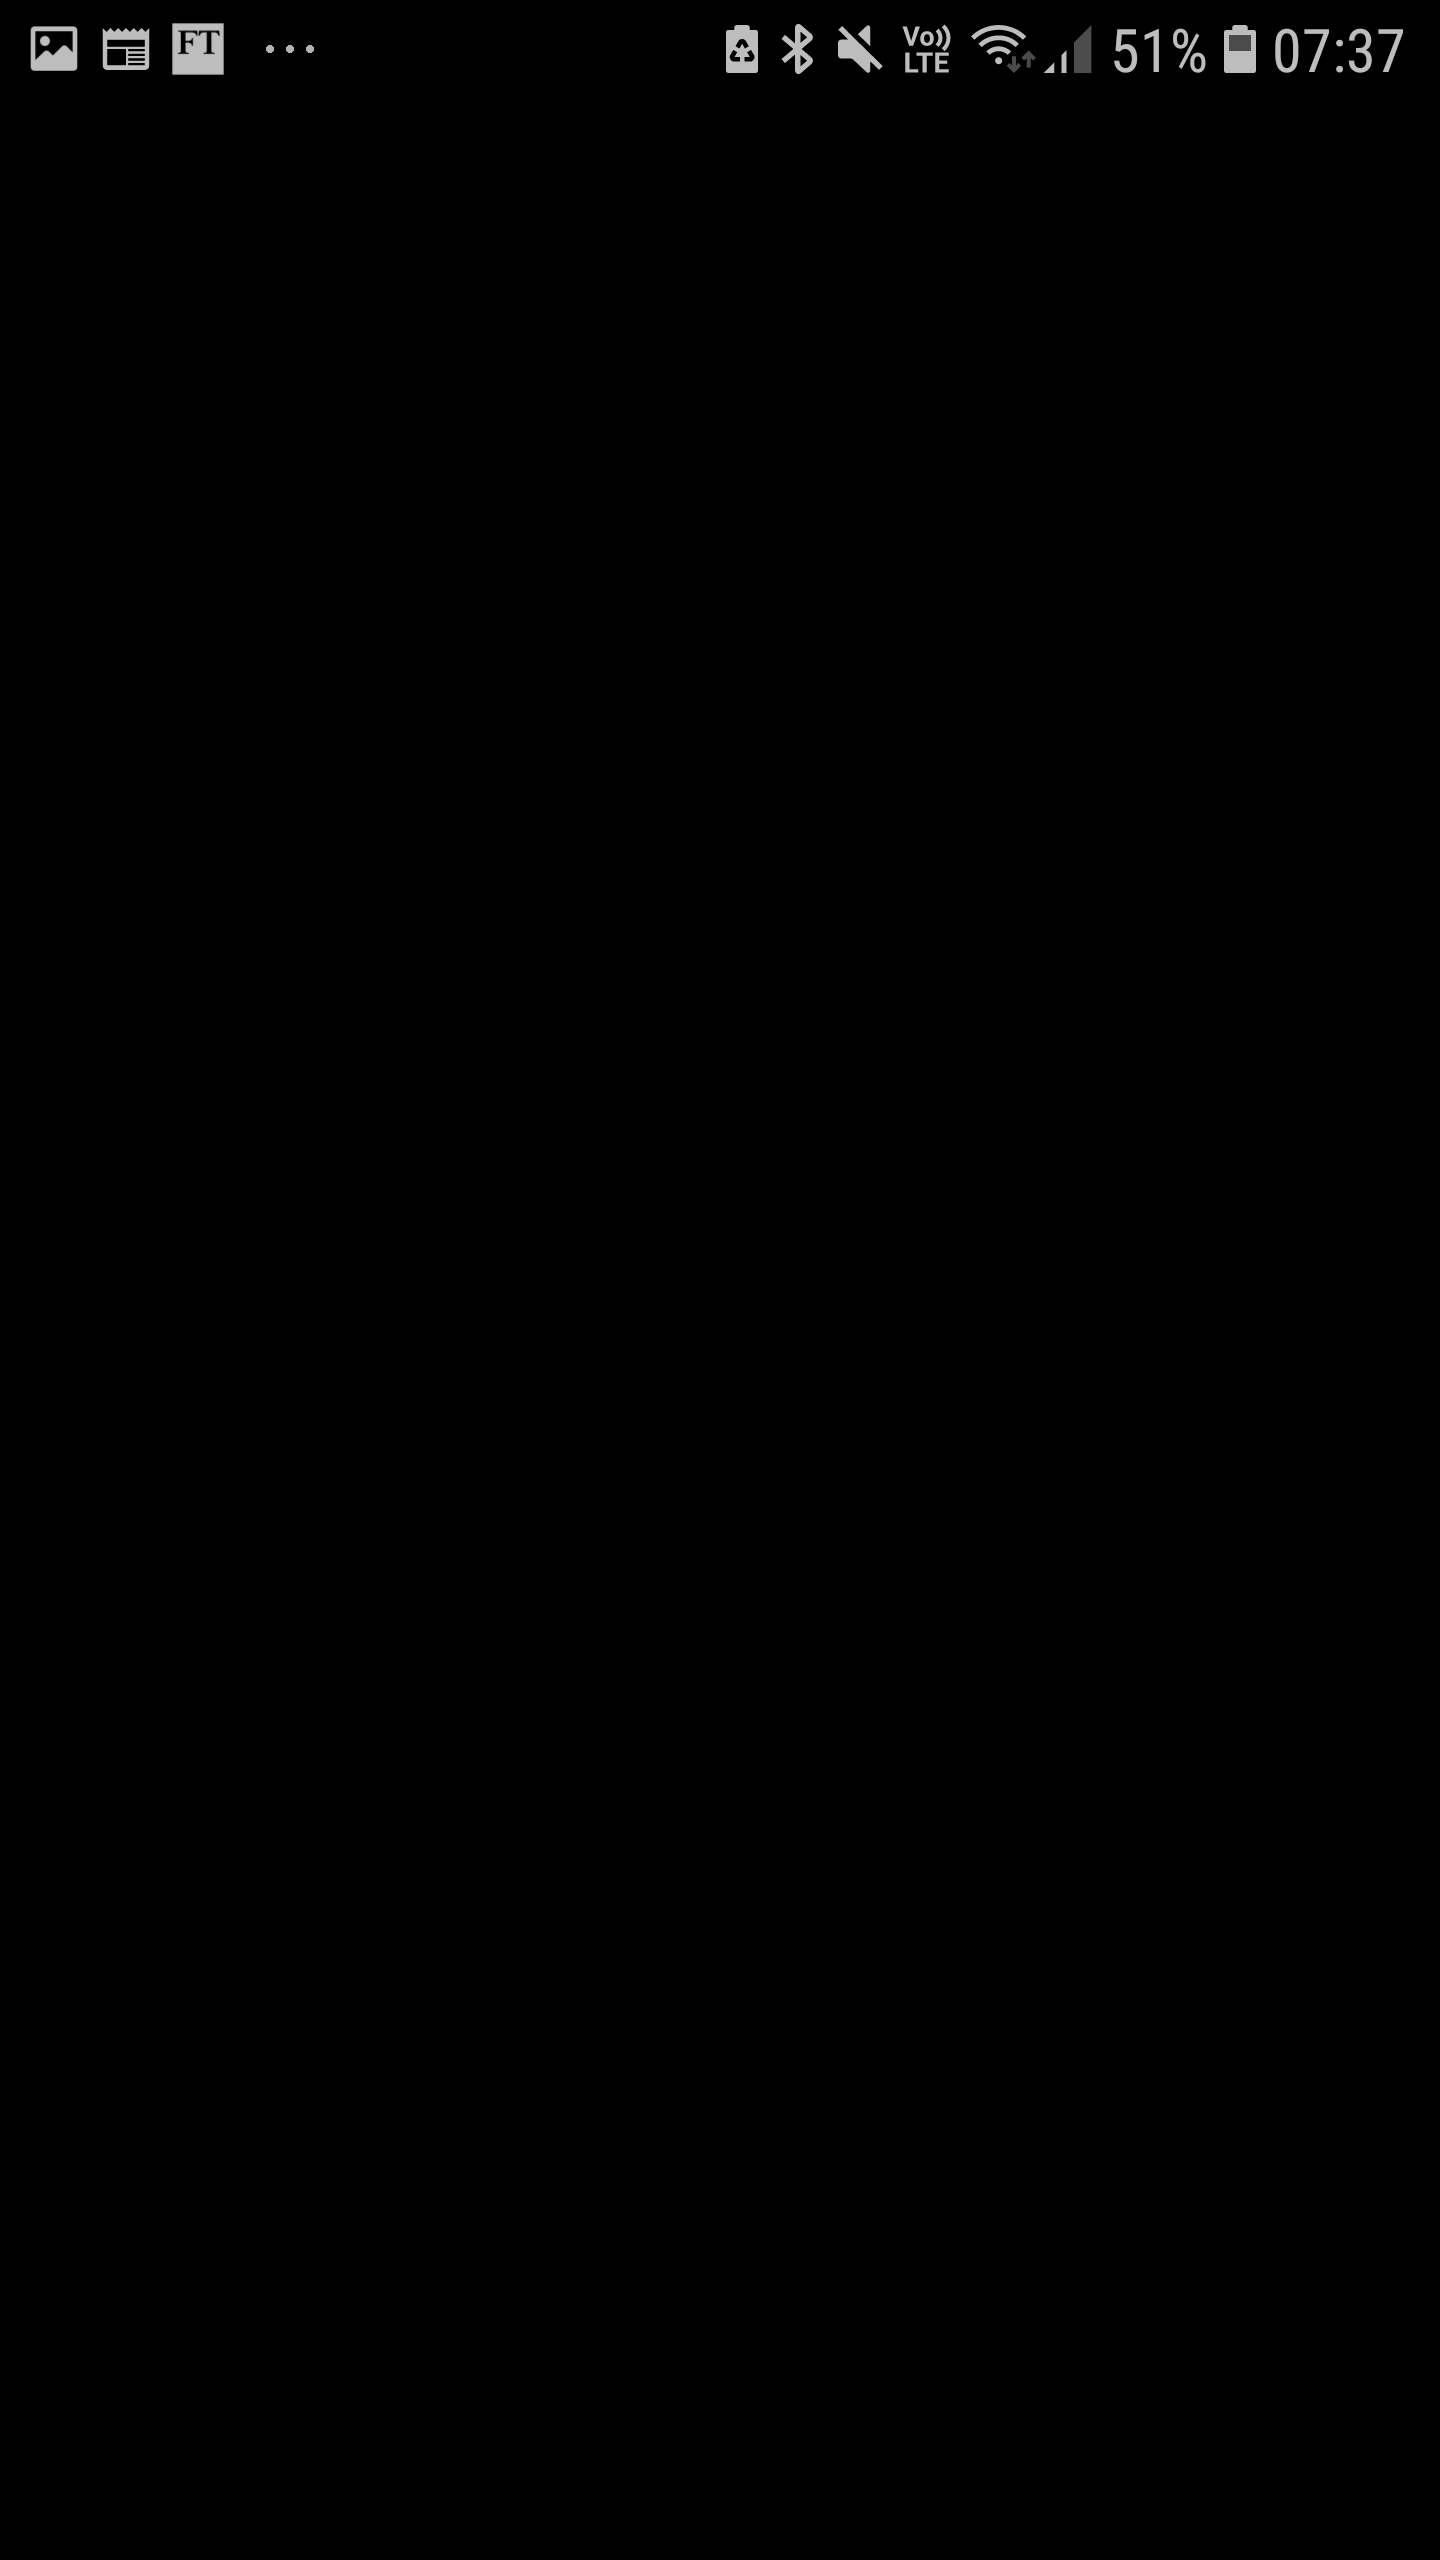
\includegraphics[width=0.45\textwidth]{images/android-screenshots/Screenshot_20200928-073727_FT.jpg}\label{fig:android_ft_GUI}}
    \hfill
    \subfloat[The FT app in the task list] {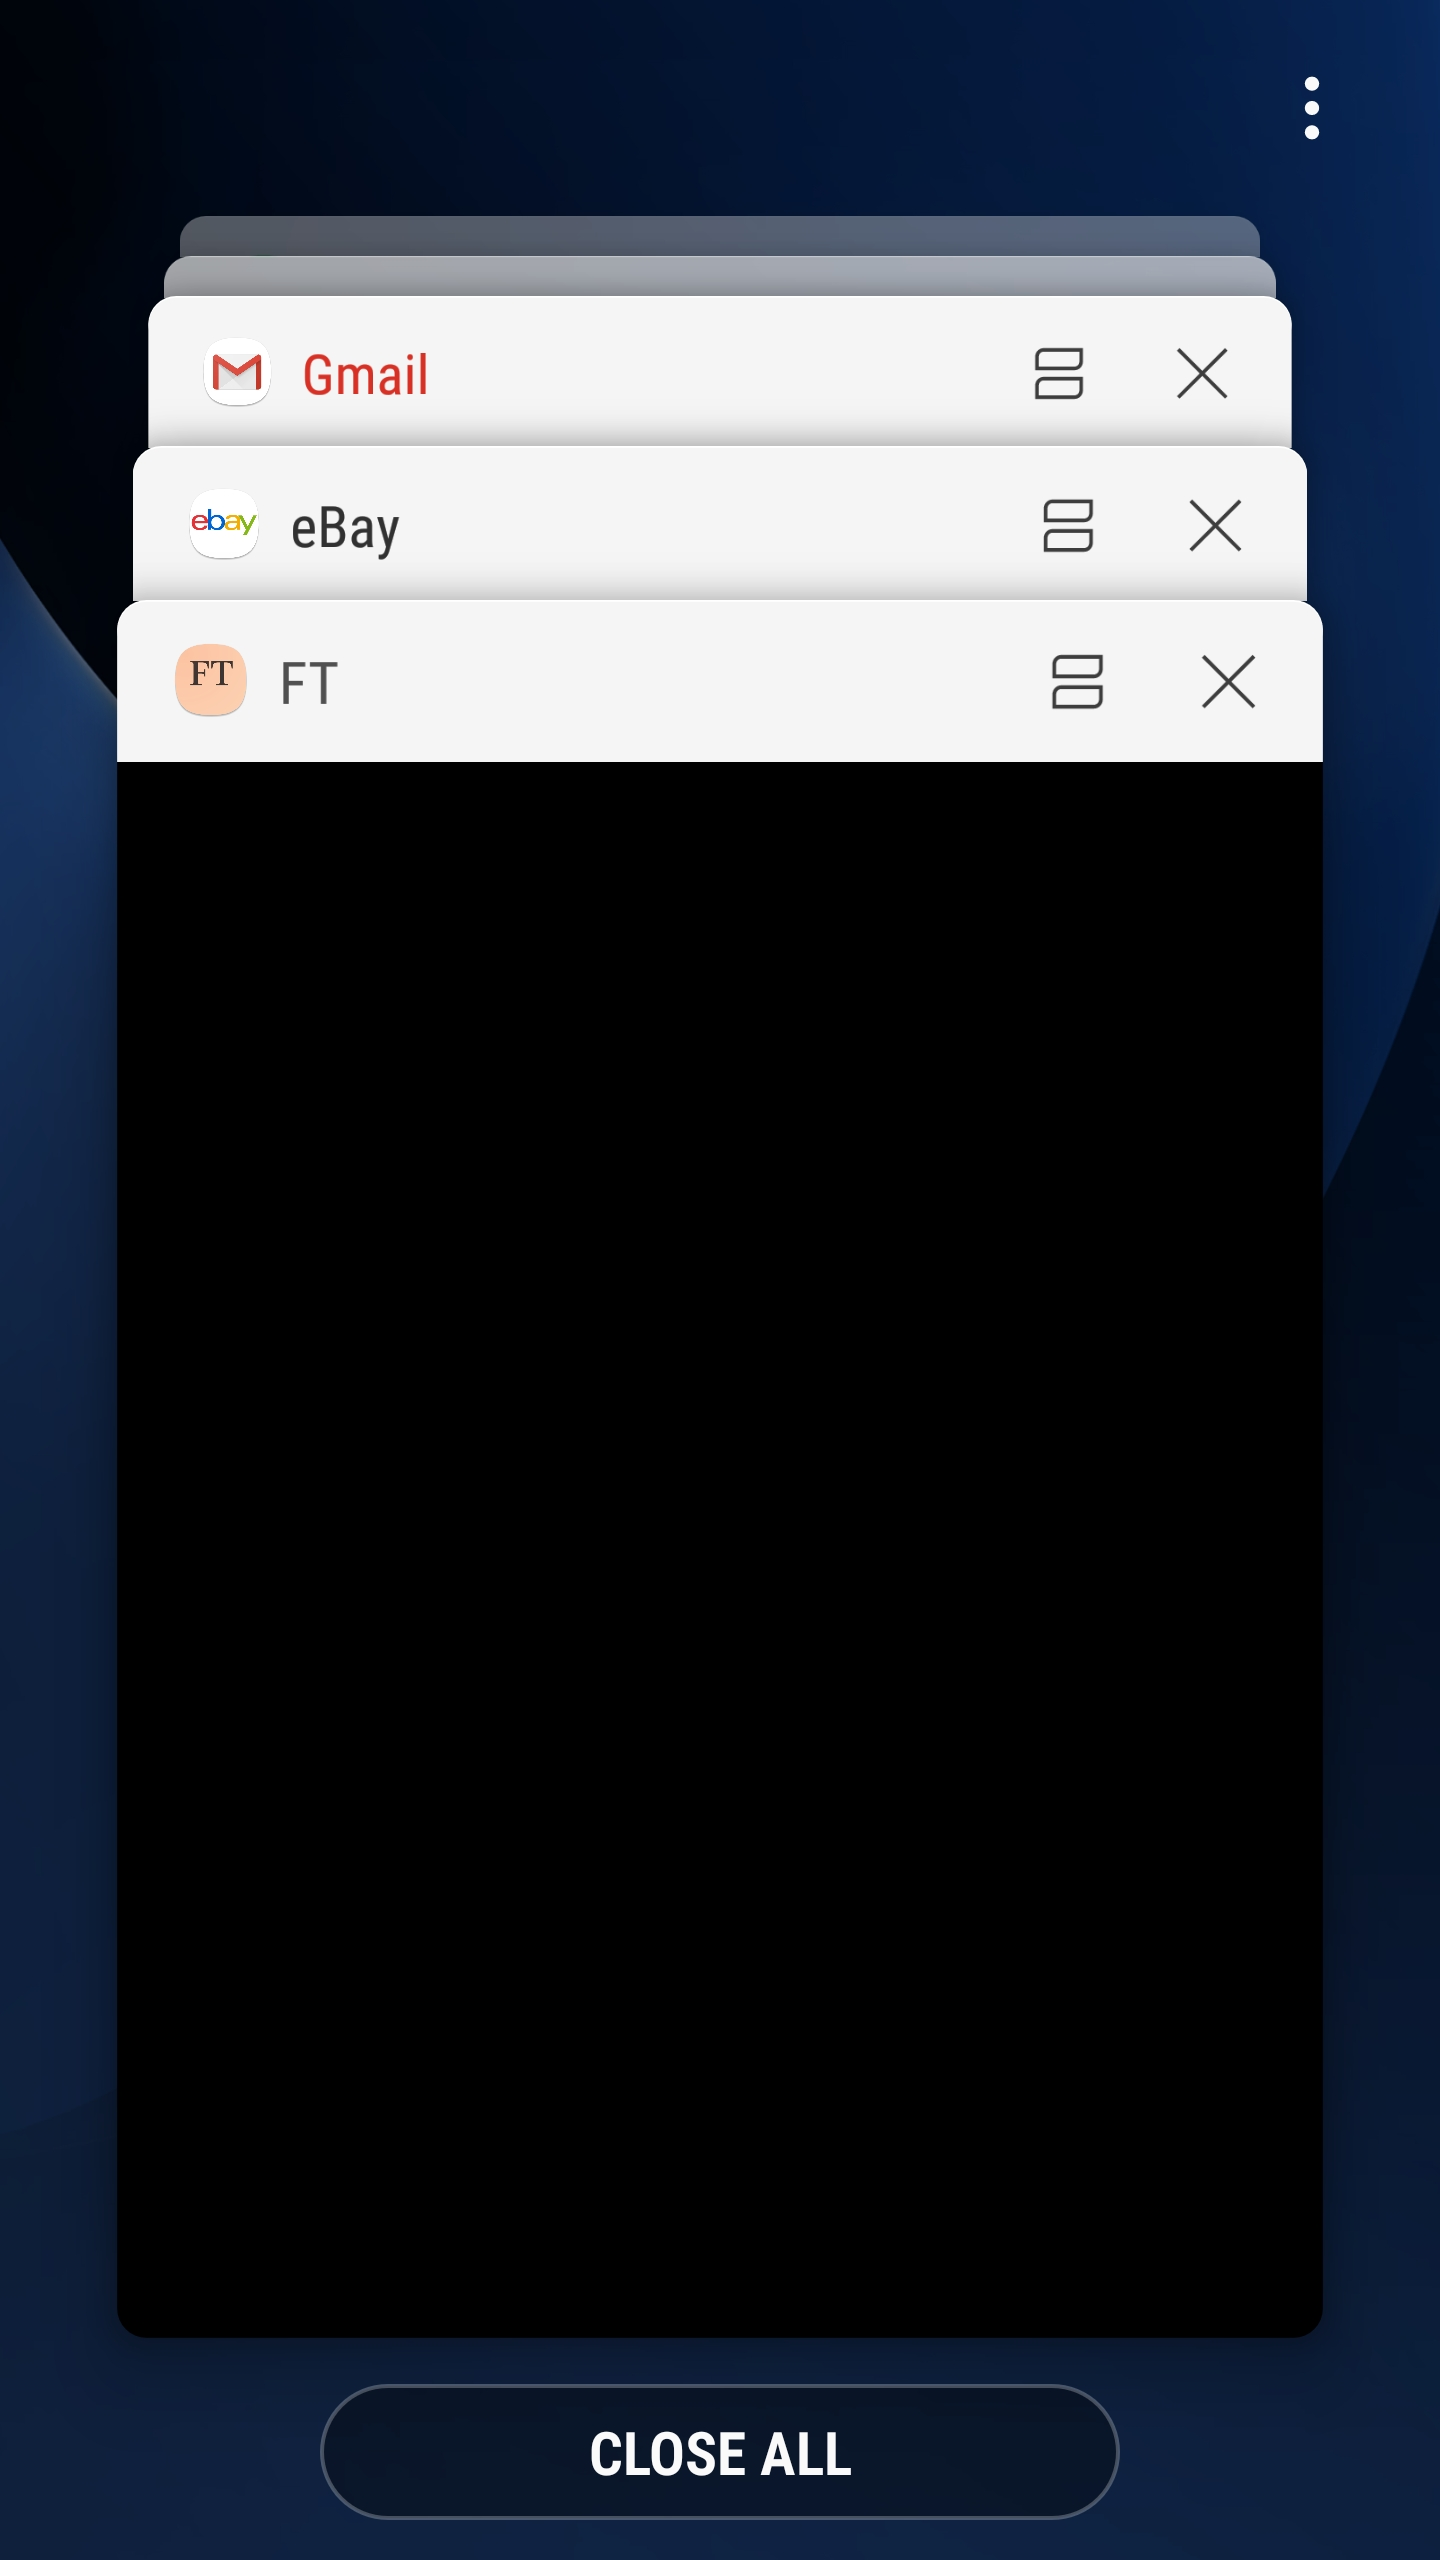
\includegraphics[width=0.45\textwidth]{images/android-screenshots/Screenshot_20200928-073745_FT.jpg}\label{fig:ft_android_app_in_task_list}}
      \caption{Black screen when notification selected}
    \label{fig:ft_android_app_bsod}
\end{figure}

\begin{figure}
    \centering
    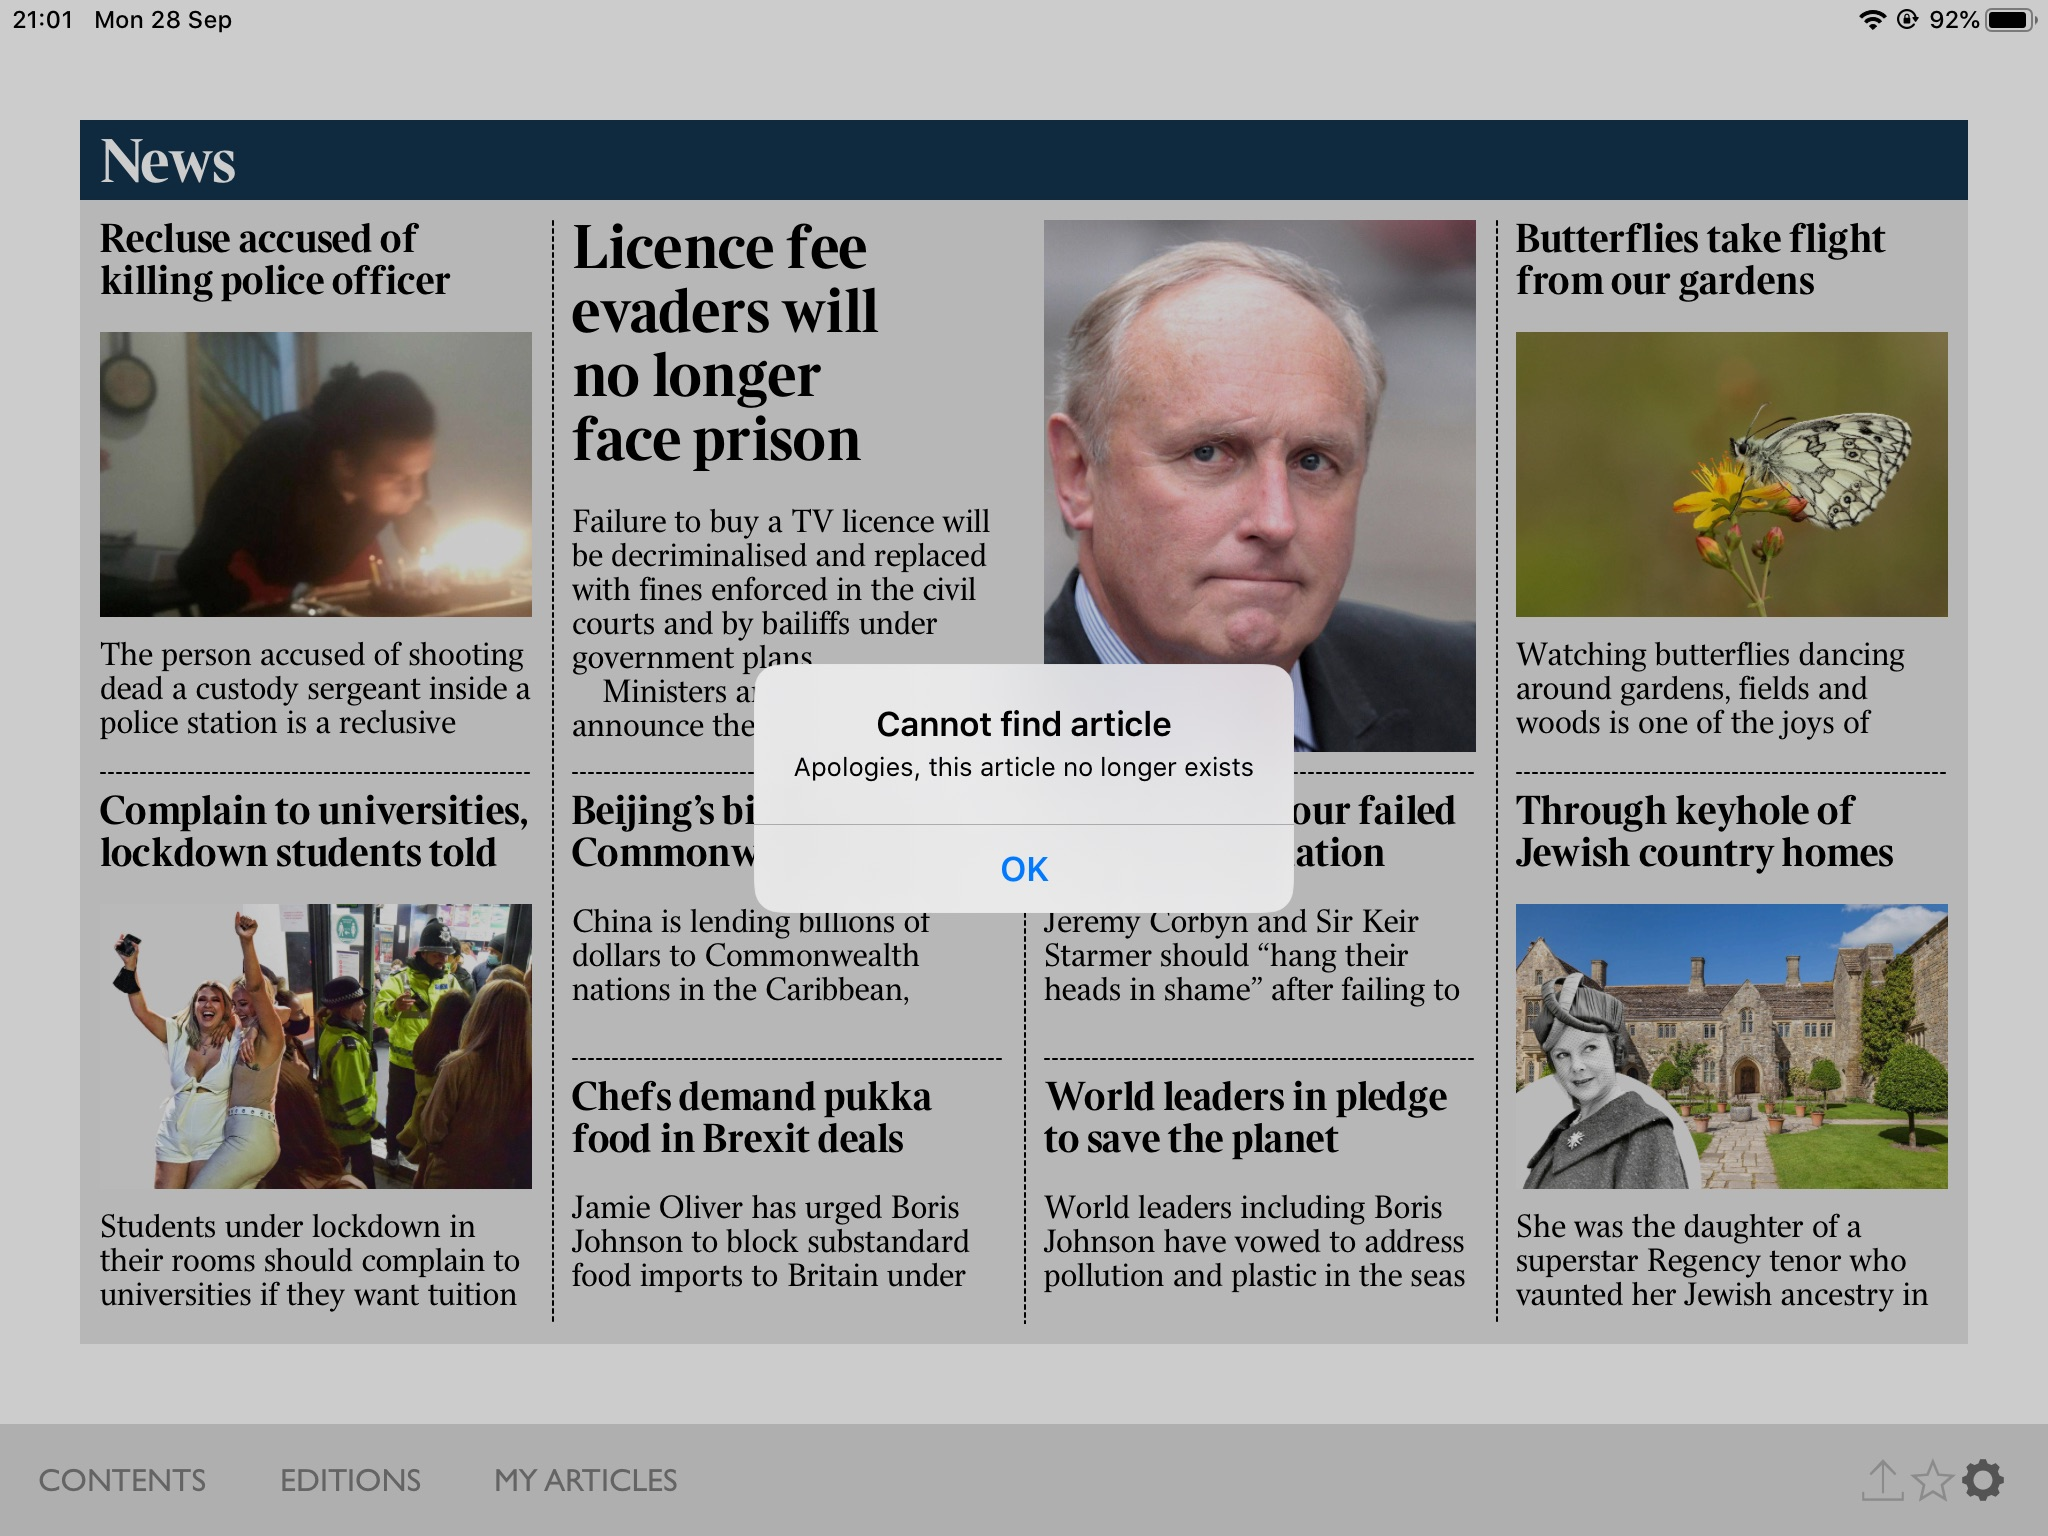
\includegraphics[width=13cm]{images/ios-screenshots/The-Times-iOS-Screenshot-2020-09-28.png}
    \caption{The Times iOS app: ``this article no longer exists" \nth{28} September 2020.}
    \label{fig:thetimes-ios-this-article-no-longer-exists}
\end{figure}

